\begin{figure}[htb]
  \centering
  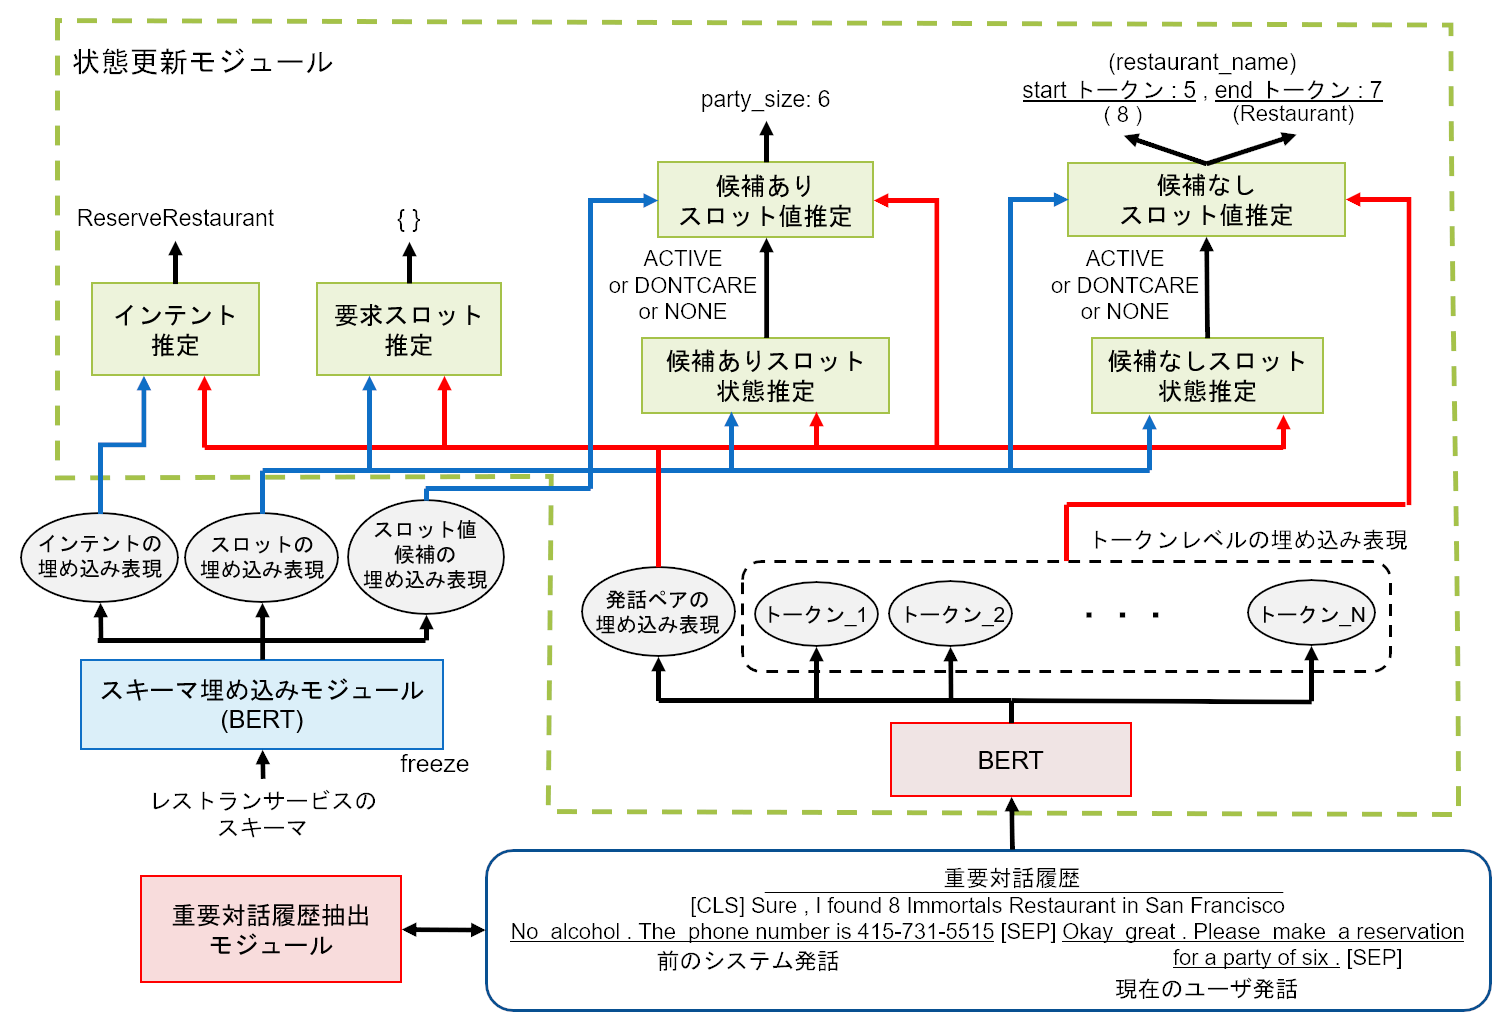
\includegraphics[width=15cm]{chapter4/teian2.eps}
  \caption{重要対話履歴抽出モジュールを加えた提案モデル}
  \label{fig:teianmodel}
\end{figure}

\begin{table}[thb]
  \centering
  \caption{SGDデータセットにある対話例の一部}
  \label{tab:taiwarei}
  \begin{tabularx}{\linewidth}{|p{55mm}|L|}\hline
    \multicolumn{1}{|c|}{
    \begin{tabular}{c}
      発話文\\(U:ユーザ,S:システム)
    \end{tabular}
    } 
    & \multicolumn{1}{|c|}{
      \begin{tabular}{c}
      対話状態(オレンジ色)or\\システムの対話行為(水色)
    \end{tabular}
     } \\ \hline \hline
     \rowcolor[rgb]{1.0,0.9,0.8}
    U1: Can you pull up a list of places to eat? & \{インテント:FindRestaurant, 要求スロット:[ ], スロット値:\{\} \}\\ \hline
    \rowcolor[rgb]{0.8, 1.0, 1.0}
    S1: Sure, what city should I search? And what kind of food would you like? & \{ REQUEST(city, [ ]), REQUEST(cuisine, [ ]) \} \\ \hline
    \rowcolor[rgb]{1.0,0.9,0.8}
    U2: Search San Francisco for Asian Fusion food & \{インテント:FindRestaurant, 要求スロット:[ ], スロット値:\{ city: San Fracisco, cuisine: Asian Fusion \} \} \\ \hline
    \rowcolor[rgb]{0.8, 1.0, 1.0}
    S2: Sure, I found 8 Immortals Restaurant in San Francisco & \{ OFFER(restaurant\_name, 8 Immortals Restaurant), OFFER(city, San Francisco) \} \\ \hline
    \rowcolor[rgb]{1.0,0.9,0.8}
    U3: Is there live music? & \{インテント:FindRestaurant, 要求スロット:[ has\_live\_music ], スロット値:\{ city: San Fracisco, cuisine: Asian Fusion \} \} \\ \hline
    \rowcolor[rgb]{0.8, 1.0, 1.0}
    S3: Unfortunately no. & \{ INFORM(has\_live\_music, False) \} \\ \hline
    \rowcolor[rgb]{1.0,0.9,0.8}
    U4: Do they serve alcohol? And what's their phone number? & \{インテント:FindRestaurant, 要求スロット:[ phone\_number, serves\_alcohol ], スロット値:\{ city: San Fracisco, cuisine: Asian Fusion \} \} \\ \hline
    \rowcolor[rgb]{0.8, 1.0, 1.0}
    S4: No alcohol. The phone number is 415-731-5515 & \{ INFORM(serves\_alocohol, False), INFORM(phone\_number, 415-731-5515) \} \\ \hline
    \rowcolor[rgb]{1.0,0.9,0.8}
    U5: Okay great. Please make a reservation for a party of six. & \{インテント:ReserveRestaurant, 要求スロット:[ ], スロット値:\{ city: San Fracisco, cuisine: Asian Fusion, party\_size: 6, restaurant\_name: 8 Immortals Restaurant \} \} \\ \hline
    \rowcolor[rgb]{0.8, 1.0, 1.0}
    \multicolumn{1}{|c|}{\vdots} & \multicolumn{1}{c|}{\vdots} \\ \hline
  \end{tabularx}
\end{table}

ベースラインモデルが過去の発話中に存在するスロット値を推定するために,対話履歴を用いる.深層学習による対話状態追跡で対話履歴を用いる場合,直近の数発話を履歴として入力に用いる\cite{trade,mrc}.しかし,直近の数発話では計算量の観点から多くの発話を入力するのは困難である.そこで,本研究では対話状態追跡に特に重要な発話をモデルへ入力するために,対話行為タグを用いた履歴抽出を提案する.この手法により,履歴として用いる発話を対話状態の推定に必要な情報を持つ発話のみにする.そのような発話を重要対話履歴とする.
\par

図\ref{fig:teianmodel}に示す提案モデルでは,ベースラインモデルの入力文を作成する箇所に重要対話履歴を抽出する重要対話履歴抽出モジュールを加えている.このモジュールは直前の最も重要度の高い履歴を1つ入力に加える.方法としては,入力文中にある前のターンのシステム発話が特定の対話行為タグを持つ場合にその発話を保持し,既に発話を保持している場合は新しい発話に更新する.そして,元々保持されていた発話を重要対話履歴として入力に加える.入力は,重要対話履歴,前のターンのシステム発話,現在のターンのユーザ発話の 3 発話となる.
\par
SGD データセットの対話例を表\ref{tab:taiwarei}に示す.表\ref{tab:taiwarei} では,n 回目のユーザ発話を Un,システム発話を Sn と表す.対話状態はユーザ発話が入力された後の状態を示していて,システムの対話行為はシステム発話に付与されているものを示している.この対話例では,S2 でシステムが提案したレストラン名に対して,U5 で了承してレストラン名が対話状態に反映される.この時,ユーザはレストラン名を過去の発話から暗黙的に参照しているため,発話中にレストラン名は含まれていない.そのため,S2 での発話を履歴として入力に加えて,レストラン名を示す “restaurant\_name” のスロット値となる “8 Immortals Restaurant” を推定可能にする必要がある.
\par
図 \ref{fig:teianmodel} では,例として表\ref{tab:taiwarei}のシステムの対話行為“OFFER”を持つ発話を抽出している.入力に加えられる重要対話履歴は,“8 Immortals Restaurant”を含む S2 での発話になる.入力文にスロット値となる文字列が含まれるため,スロット値として抜き出すことが可能になる.直近の数発話を対話履歴として用いる従来手法の場合は,直近の 6 発話を入力に加える必要があるが,提案手法では 3 発話で推定が行える.また,図\ref{fig:teianmodel}では5ターン前の発話を抽出しているが,提案手法はさらに前の発話を抽出することも可能である.ゆえに,提案手法は計算量の削減と同時に性能の向上が期待できる.